\section{Ambiente de Desenvolvimento}

\begin{frame}[fragile]{Teclado APL}

    Para inserir os glifos APL, é preciso ou um teclado especializado ou a instalação de um \textit{layout} compatível.
        \pause

    \begin{figure}
        \centering
        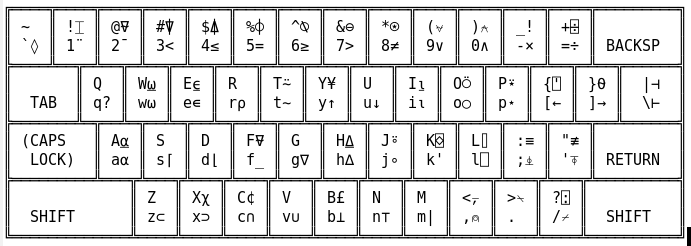
\includegraphics[scale=0.5]{figs/keyboard.png}

        \caption{\textit{Layout} de teclado GNU APL. Fonte: \href{https://lists.gnu.org/archive/html/bug-apl/2014-06/msg00261.html}{Bug-apl}}
    \end{figure}

\end{frame}

\begin{frame}[fragile]{Configuração de Layout no Ubuntu 20.04}

    \begin{enumerate}
        \item Nas configurações do sistema (\textit{Settings}), escolha a opção de região e
            linguagem (\textit{Region \& Language})
        \pause

        \item Adicione um segundo \textit{layout} qualquer (por exemplo, o \textit{layout} Braile)
            usando o símbolo \texttt{+} na lista de entradas (\textit{Input Sources})
        \pause

        \item Rode, no seu terminal, o comando

            \inputsyntax{bash}{codes/setlayout.sh}
        \pause

        \item Para tornar esta configuração permanente, adicione esta linha ao arquivo
            \texttt{~/.bashrc}
        \pause

        \item Além do \textit{layout}, é recomendada a instalação da fonte \texttt{APL 385} para
            melhor visualização dos glifos
    \end{enumerate}
\end{frame}

\begin{frame}[fragile]{Inserção de glifos APL}

    \begin{itemize}
        \item Uma vez disponível o \textit{layout} APL, os glifos podem ser inseridos por meio
            de um combinação de teclas
        \pause

        \item A tecla \texttt{APL} deve ser combinada com uma outra tecla, ou com a tecla
            \texttt{Shift} e outra tecla
        \pause

        \item No \textit{layout} proposto, a tecla \texttt{APL} corresponde a tecla
            \texttt{Alt Gr}
        \pause

        \item Por exemplo, os glifos \texttt{⍴} e \texttt{⍒} podem ser inserido por meio das combinações
            \texttt{APL+p} e \texttt{APL+Shift+3}, respectivamente

        \pause

        \item Uma maneira alternativa é inserir os códigos unicode de cada caractere diretamente
            em seu editor

        \pause

        \item Este método dispensa a configuração do \textit{layout}, porém demanda a memorização
            dos códigos e do uso de mais teclas por caractere
    \end{itemize}

\end{frame}
%- é preciso instalar um teclado APL: https://stackoverflow.com/questions/68065520/add-apl-keyboard-layout-on-linux-20-04
%    * Adicione um segundo layout extra (Braile, por exemplo, em System -> Region & Language
%    * adicione esta linha no .bashrc
%        setxkbmap -layout br,apl -variant ,dyalog -option grp:switch
%    * A tecla alt right, quando pressionada, mudará entre os dois layouts possíveis
%
%- para encerrar, é preciso chamar a funçã off (quad + off, com quad = right atl + l) https://help.dyalog.com/12.0/index.html?page=html%2Fexit%20from%20apl.htmac


